\documentclass{article}
\usepackage{color}
\usepackage{xcolor}
\usepackage{amsmath}
\usepackage[thinlines]{easytable}
\usepackage{graphicx}
\usepackage{enumitem}
\usepackage{listings}
\usepackage{geometry}

% Tikz stuff
\usepackage{tikz}
\usepackage{tikz-qtree}
\usepackage{tikz-qtree-compat}
\usetikzlibrary{positioning}

\tikzset{blue node/.style={circle,fill=blue!20,draw,minimum size=1cm,inner sep=0pt},}
\tikzset{red node/.style={circle,fill=red!20,draw,minimum size=1cm,inner sep=0pt},}
\tikzset{green node/.style={circle,fill=green!20,draw,minimum size=1cm,inner sep=0pt},}
\tikzset{yellow node/.style={circle,fill=yellow!20,draw,minimum size=1cm,inner sep=0pt},}

\tikzset{graph node/.style={circle,fill=orange!30,draw,minimum size=1cm,inner sep=0pt},}

% Fancy code block wider than margins

\makeatletter
\newcommand*{\centerfloat}{%
  \parindent \z@
  \leftskip \z@ \@plus 1fil \@minus \textwidth
  \rightskip\leftskip
  \parfillskip \z@skip}
\makeatother

\title{COS 485 --- Homework 5}

\author{Samuel Barton \and Benjamin Montgomery}

\date{April 3, 2017}

\begin{document}
	\maketitle
	\section*{Problem 1}

In this problem we categorize the following sorting algorithms into the
various genres of algorithms discussed in this course.
\\
\\
By definition, iterative improvement gradually improves an initial solution.
Thus it is impossible for a sorting algorithm to be an iterative improvement 
algorithm as a list is either sorted or unsorted. Once there is a solution,  no
improvements can be made on it.
\\
\\
\begin{tabular}{l c p{6cm}}
        \textbf{Algorithm} & \textbf{Technique} & \textbf{Justification} \\
        \hline
    Insertion sort & Greedy & Go through each element starting at position 0. Shift all of the elements greater than the current one to the left.\\
    Selection sort & Greedy & Find the smallest item in the unsorted part of the list and append it to the end of the sorted part. \\
    Bubble sort & Greedy & If the next value is smaller than the current one, swap them.\\
    Quicksort & Divide and Conquer & Divide the problem size recursively, sort at the bottom, then sort on your way up. Note that Quicksort \textit{can} be implemented with a randomized partition.\\
    Merge sort & Divide and Conquer & Divide the problem size recursively, sort at the bottom, then sort on your way up.\\
    Heap sort & Greedy & Larger values go higher (maxheap), or smaller values go higher (minheap)\\
\end{tabular}

	\section*{Problem 2}

In this problem we consider the case of one miserly king who has 
demanded a weighing of $N$ coins with the understanding that one coin
is counterfeit and lighter than the others. 
\\
\\
The algorithm to effeciently solve this is as follows:
\begin{enumerate}[noitemsep]
    \item divide coins into three parts $A$, $B$, and $C$. $A$ and $B$
          to be divided into a multiple of three, and the rest are left
          in $C$ 
    \item weigh two of them
    \subitem if $A = B$,  then throw out $A$ and $B$ and keep $C$
    \subitem if $A < B$, then throw out $B$ and $C$ and keep $A$
    \subitem if $B < A$, then throw out a and $C$ and keep $B$
    \item repeat
\end{enumerate} 

In the end, N wasn't divisible by 3, then we will have either 1 or two 
extra to deal with. If there is one extra, then we do two comparisons. 
If there are two extra left then we still do two comparisons.
\\
\\
In the worst case, we do $\lceil \; \log_3 N \; \rceil + 1$ comparisons.

	\pagebreak
	\section*{Problem 3}

It is stated that both problem $A$ and problem $B$ are decision problems such that $A \propto B$. It is also stated that $A$ is an NP-complete problem. We are then asked if $B$ is also $NP$-Complete.

We observe that $B$ has two possibilities:
\begin{enumerate}
    \item $B$ is in $P$. This means $A \propto_T B$, so $B$ is $NP$-hard. This means that $P = NP$, so $B$ is in $NP$.
    \item $B$ is not in $P$. This means $B$ is at least in $NP$. It is stated all problems in $NP$ can be reduced to $NP$-hard problems.
\end{enumerate}

Both of the above indicate that $B$ is an $NP$-complete problem.
	\pagebreak
	\section*{Problem 4}
In order to have a worst-case linear algorithm for finding the mode in an array, consider the following algorithm:
\begin{enumerate}
    \item Create an empty HashMap in the form of $K$, $V$. The type of $K$ is the same as that of the array values, and the type of $V$ is an integer, used to count the number of occurrences of that key.
    \item Perform a linear pass on our array. For each element, check to see if it is in our HashMap as a key.
        \subitem If it is not in our HashMap, put in the element as the key, and set the HashMap's value to 1 to indicate 1 occurrence.
        \subitem If it is in our HashMap, increase the associated value in the HashMap by one, to indicate one more occurrence than before.
    \item Perform a linear pass across the set of entries in the HashMap, keeping track of the entry with the largest value. This entry holds the element that is the mode as the key, and the number of times it occurred as the value.
\end{enumerate}

Our analysis is as follows:\\
\begin{enumerate}
    \item Creation of the \textbf{empty} HashMap is $O(1)$.
    \item Our linear pass across the array is, by construction, $T_n = n$. At each element, we perform an $O(1)$ \textit{get} operation. We then perform another $O(1)$ insertion, whether it be an entry that gets inserted, or an existing value that gets updated. This is a total of $T_n = 3n$
    \item Our linear pass across the set of entries in the HashMap is also  $T_n = n$. In the worst case, there are $N$ entries, so we check $n$ times in total if we have a new max. This is a total of $T_n = 2n$.
\end{enumerate}
Therefore, we can express our time complexity as the following:
\\
$$
    T_n = O(1) + 3n + 2n \implies T_n \in \Theta(n)
$$
	\section*{Problem 5}

In this problem we are given the following situation and asked to find the 
minimun number of afternoons required to solve it.

\begin{quote}
    A list of 17 committees with 200 unique members where no member can be in more
    than 5 committees. Each committee meeting takes one afternoon to complete.
\end{quote}
%
This problem is most similar to the graph coloring problem. We cast this problem
into the graph coloring problem in the following way:
\\
\\
First, each job becomes a vertex in the graph. Each edge in the graph represents a
conflicting committee, namely a pair of committees which share a member. In order 
to determine whether a pair of committees conflict we take a linear pass through 
their respective membership lists and look for a common member.
\\
\\
With this graph built we simply run the graph coloring algorithm and return the 
minimun number of colors needed to color the graph. This number is the number of 
afternoons needed to hold all of the meetings with no conflicts.
\begin{center}
To demonstrate this algorithm we consider the following example: 
\\\hfill
\\
    \begin{tabular}{| c | c  c  c| c c | }
        \hline
        \textbf{Committee} & \multicolumn{3}{l|}{\textbf{Members}} & 
        \multicolumn{2}{l|}{\textbf{Conflicts With}} \\
        \hline
        W & A & C & & X & Y \\
        \hline
        X & C & D & & W & Z \\
        \hline
        Y & A & B &E& W & Z \\
        \hline
        Z & B & D & & X & Y \\
        \hline
    \end{tabular}
\end{center}
%
Where we note that we are given that the optimal solution takes two afternoons. 
Below we present the graph representing these committees and the conflicts between
them.
\\
\begin{center}
    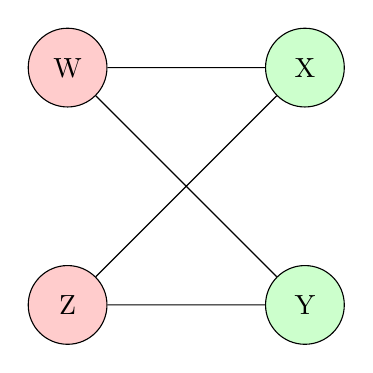
\begin{tikzpicture}
       \node[red node] (1) {W};
       \node[green node] (2) [right = 2cm of 1]{X};
       \node[green node] (3) [below = 2cm of 2]{Y};
       \node[red node] (4) [below = 2cm of 1]{Z};

       \draw (1) -- (2) 
             (1) -- (3)
             (2) -- (4)
             (3) -- (4);
    \end{tikzpicture}
\end{center}
%
Note that this is a valid coloring for the graph, and that there are two colors
needed to color this graph. This means that, by our algorithm statement, we 
can schedule all of the meetings in two afternoons with no conflicting meetings.

	\section*{Problem 6}

In this problem we are asked to find the largest set of disjoint paths
between two verticies in a graph.
\\
\\
The algorithm we propose is as follows:

\begin{enumerate}[noitemsep]
    \item Give each path in the graph a weight of 1
    \item Use Dijkstra's algorithm to find the shortest path between 
          the two target verticies
    \item Remove the edges that consititute the path found in 2, and 
          add the path to the set of disjoint paths between the two 
          verticies
    \item Repeat 1-3 until a path between the two verticies cannot be
          found
\end{enumerate}
%
Now in the worst case, which occurs when the graph is completely 
connected, there will be $V - 1$ paths between the two target verticies.
Since Dijkstra's algorithm takes $T_n \in \Theta(V \, \lg E)$ time at 
each iteration, and there will be $V - 1$ iterations to find all the
paths, then this algorithm will take
$$
T_n = (V - 1) \cdot V \, \lg E \; = \; (V^2 - V) \, \lg E = 
V^2 \, \lg E - V \, \lg E
$$ 
Thus in the worst case the algorithm's time complexity is 
$$T_n \in \Theta(V^2 \, \lg E)$$

	\section*{Problem 7}

In this problem we demonstrate, in great detail, the execution of the Hamiltonian Circuit algorithm on the graph below. On this graph we have denoted the path taken by the circuit. See the next page for the state-space tree for this circuit.

\begin{center}
    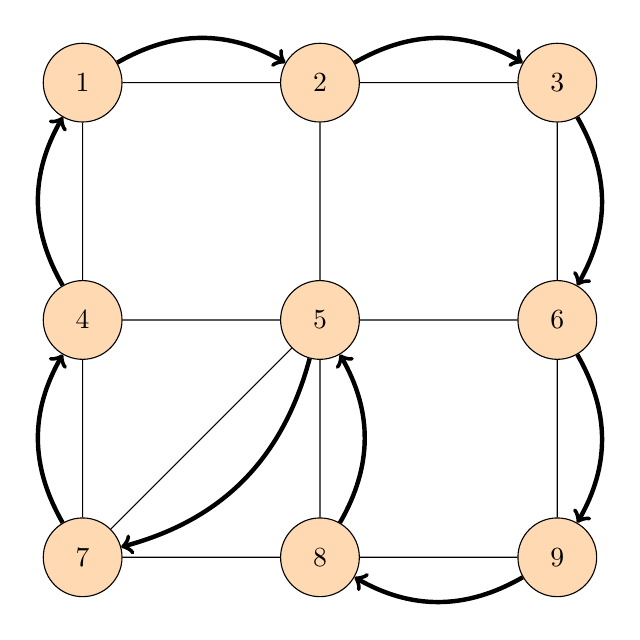
\begin{tikzpicture}
       \node[graph node] (1) {$1$};
       \node[graph node] (2) [right = 2cm of 1]{$2$};
       \node[graph node] (3) [right = 2cm of 2]{$3$};
       
       \node[graph node] (4) [below = 2cm of 1]{$4$};
       \node[graph node] (5) [right = 2cm of 4]{$5$};
       \node[graph node] (6) [right = 2cm of 5]{$6$};
       
       \node[graph node] (7) [below = 2cm of 4]{$7$};
       \node[graph node] (8) [right = 2cm of 7]{$8$};
       \node[graph node] (9) [right = 2cm of 8]{$9$};
       
       \draw
       (1) -- (2) -- (3)
       (1) -- (4) -- (7)
       (2) -- (5) -- (8)
       (3) -- (6) -- (9)
       (4) -- (5) -- (6)
(7) -- (8) -- (9)
       (7) -- (5);
	   
	   \draw [ultra thick,->,bend left=30] (1) to (2);
	   \draw [ultra thick,->,bend left=30] (2) to (3);
	   \draw [ultra thick,->,bend left=30] (3) to (6);
	   \draw [ultra thick,->,bend left=30] (6) to (9);
	   \draw [ultra thick,->,bend left=30] (9) to (8);
	   \draw [ultra thick,->,bend right=30] (8) to (5);
	   \draw [ultra thick,->,bend left=30] (5) to (7);
	   \draw [ultra thick,->,bend left=30] (7) to (4);
	   \draw [ultra thick,->,bend left=30] (4) to (1);	   	   	   	   	   	   
    \end{tikzpicture}
\end{center}

\pagebreak

\begin{center}
	\vspace*{-4cm}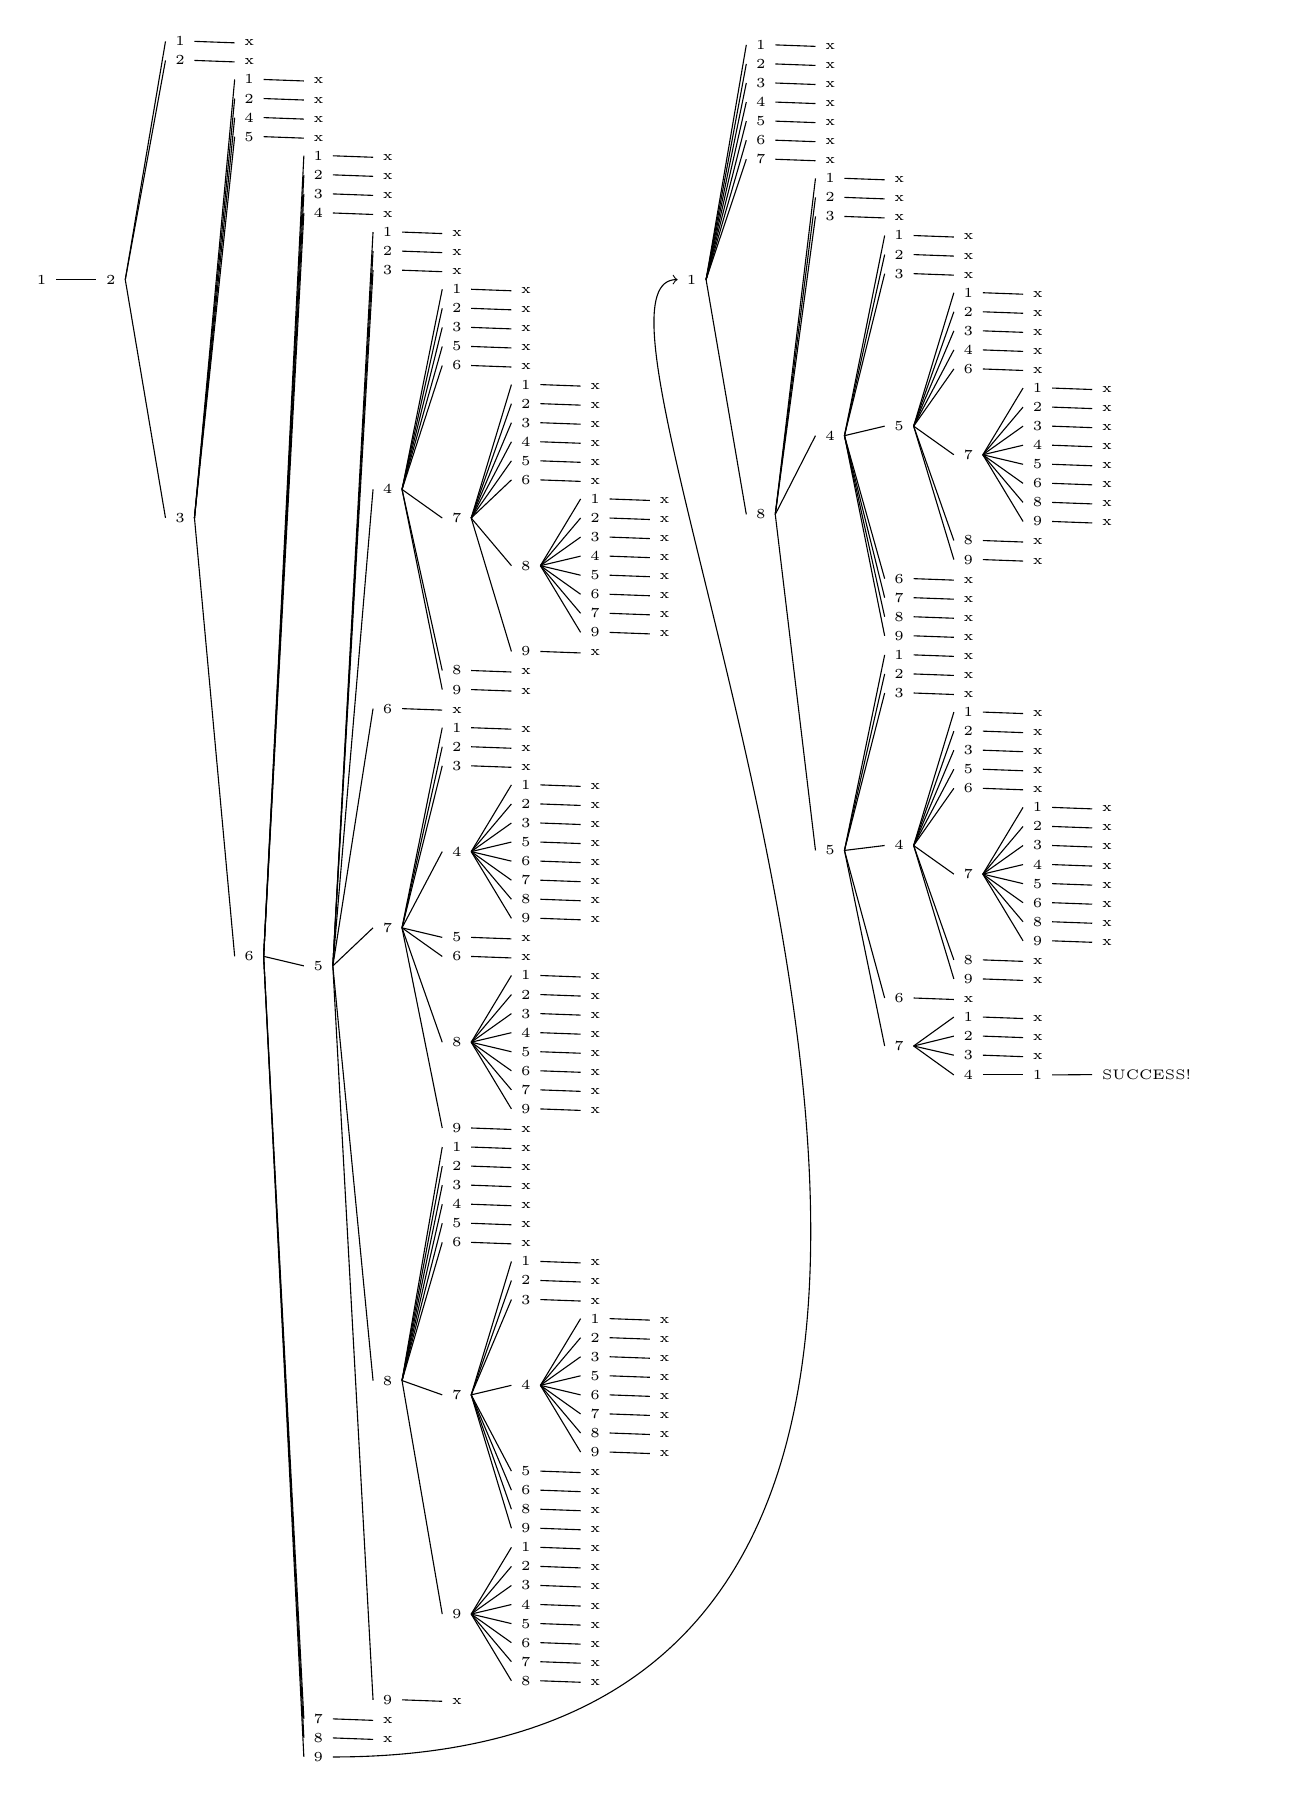
\begin{tikzpicture}[font=\tiny]
	\tikzset{grow'=right,level distance=25pt,sibling distance=-3pt}
%	\tikzset{execute at begin node=\strut}
	\tikzset{every tree node/.style={align=center,anchor=base west}}		

\Tree 
[.1 
	[.2 
		[.1 
			x
		] 
		[.2 
			x
		]
		[.3
			[.1
				x
			]
			[.2
				x
			]
			[.4
				x
			]
			[.5
				x
			]
			[.6
				[.1
					x
				]
				[.2
					x
				]
				[.3
					x
				]
				[.4
					x
				]
				[.5
					[.1
						x
					]
					[.2
						x
					]
					[.3
						x
					]
					[.4
						[.1
							x
						]
						[.2
							x
						]
						[.3
							x
						]
						[.5
							x
						]
						[.6
							x
						]
						[.7
							[.1
								x
							]
							[.2
								x
							]
							[.3
								x
							]
							[.4
								x
							]
							[.5
								x
							]
							[.6
								x
							]
							[.8
								[.1
									x
								]
								[.2
									x
								]
								[.3
									x
								]
								[.4
									x
								]
								[.5
									x
								]
								[.6
									x
								]
								[.7
									x
								]
								[.9
									x
								]
							]
							[.9
								x
							]
						]
						[.8
							x
						]
						[.9
							x
						]
					]
					[.6
						x
					]
					[.7
						[.1
							x
						]
						[.2
							x
						]
						[.3
							x
						]
						[.4
							[.1
								x
							]
							[.2
								x
							]
							[.3
								x
							]
							[.5
								x
							]
							[.6
								x
							]
							[.7
								x
							]
							[.8
								x
							]
							[.9
								x
							]
						]
						[.5
							x
						]
						[.6
							x
						]
						[.8
							[.1
								x
							]
							[.2
								x
							]
							[.3
								x
							]
							[.4
								x
							]
							[.5
								x
							]
							[.6
								x
							]
							[.7
								x
							]
							[.9
								x
							]
						]
						[.9
							x
						]
					]
					[.8
						[.1
							x
						]
						[.2
							x
						]
						[.3
							x
						]
						[.4
							x
						]
						[.5
							x
						]
						[.6
							x
						]
						[.7
							[.1
								x
							]
							[.2
								x
							]
							[.3
								x
							]
							[.4
								[.1
									x
								]
								[.2
									x
								]
								[.3
									x
								]
								[.5
									x
								]
								[.6
									x
								]
								[.7
									x
								]
								[.8
									x
								]
								[.9
									x
								]
							]
							[.5
								x
							]
							[.6
								x
							]
							[.8
								x
							]
							[.9
								x
							]
						]
						[.9
							[.1
								x
							]
							[.2
								x
							]
							[.3
								x
							]
							[.4
								x
							]
							[.5
								x
							]
							[.6
								x
							]
							[.7
								x
							]
							[.8
								x
							]
						]
					]
					[.9
						x
					]
				]
				[.7
					x
				]
			    [.8
					x
				]
			    [.\node(site){$9$}; ]
			]
		] 
	] 
]

\begin{scope}[shift={(3.25in,0in)}]
\Tree
[.\node(root){$1$}; 
	[.1
		x
	]
	[.2
		x
	]
	[.3
		x
	]
	[.4
		x
	]
	[.5
		x
	]
	[.6
		x
	]
	[.7
		x
	]
	[.8
		[.1
			x
		]
		[.2
			x
		]
		[.3
			x
		]
		[.4
			[.1
				x
			]
			[.2
				x
			]
			[.3
				x
			]
			[.5
				[.1
					x
				]
				[.2
					x
				]
				[.3
					x
				]
				[.4
					x
				]
				[.6
					x
				]
				[.7
					[.1
						x
					]
					[.2
						x
					]
					[.3
						x
					]
					[.4
						x
					]
					[.5
						x
					]
					[.6
						x
					]
					[.8
						x
					]
					[.9
						x
					]
				]
				[.8
					x
				]
				[.9
					x
				]
			]
			[.6
				x
			]
			[.7
				x
			]
			[.8
				x
			]
			[.9
				x
			]
		]
		[.5
			[.1
				x
			]
			[.2
				x
			]
			[.3
				x
			]
			[.4
				[.1
					x
				]
				[.2
					x
				]
				[.3
					x
				]
				[.5
					x
				]
				[.6
					x
				]
				[.7
					[.1
						x
					]
					[.2
						x
					]
					[.3
						x
					]
					[.4
						x
					]
					[.5
						x
					]
					[.6
						x
					]
					[.8
						x
					]
					[.9
						x
					]
				]
				[.8
					x
				]
				[.9
					x
				]
			]
			[.6
				x
			]
			[.7
				[.1
					x
				]
				[.2
					x
				]
				[.3
					x
				]
				[.4
					[.1
						SUCCESS!
					]
				]
			]
		]
	]
]
\end{scope}
\draw[<-](\subtreeof{root}.133.2) ..
controls +(west:2) and +(east:12)..(site);

	\end{tikzpicture}
\end{center}
	\section*{Problem 8}

In this problem we are asked to construct a branch and bound algorithm to solve the ``sequence alignment'' problem from Section 3.7 of the text. In this problem, we have the following. We are trying to align two sequences to minimize the overall ``cost'' of the resulting aligned sequence pair. The ``cost'' is measured using the following metric: A mismatch between two elements in the aligned pair has a cost of 1, and a gap in the aligned sequence has a cost of 2.
\\
\\
There are three possibilities for each pair we must align: we take an element from both sequences, take one from the top seqence and put a gap in the bottom sequence, or we put a gap in the top sequence and take an element from the bottom sequence. The three possibilities are shown below.

\begin{center}
	\begin{minipage}{0.3\textwidth}
	\centering
	\begin{tabular}{c}	
		{\large \textbf{X}} \\
		{\large \textbf{Y}} \\
	\end{tabular}
	\end{minipage}
	\begin{minipage}{0.3\textwidth}
		\centering
	\begin{tabular}{c}
		{\large \textbf{X}} \\
		{\large \textbf{-}} \\
	\end{tabular}
	\end{minipage}
	\begin{minipage}{0.3\textwidth}
		\centering
	\begin{tabular}{c}
		{\large \textbf{-}} \\
		{\large \textbf{Y}} \\
	\end{tabular}
	\end{minipage}
\end{center}

We do not consider the case of not taking an element from either sequence as it does not advance the solution. 
The greedy solution is an initial bound. The greedy solution is defined as taking both sequences until one runs out and then inserting blanks until the longer sequence has been exhausted as well. 
\\
\\
Our algorithm is as follows. For each pair we are to align, we consider the three possibilities and take the one with the least cost, keeping track of the total cost thus far as we go. If at any point we overstep the bound, then we backtrack to the previous pair and try the next lowest cost option until we run out of possibilities. As soon as we find a solution cheaper than the current bound, we update the bound with the cost of the new solution.
\\
\begin{center}
	{\large \textbf{Analysis}}
\end{center}

The state space vector for our algorithm is the familiar set as seen in many other backtracking algorithms.
$$
	\{ C_1,\,C_2,\,...,C_n \}
$$
In this case, $n$ is the length of the longest sequence.
\\
\\
Our algorithm has three possibilities per choice, and we are required to explore all possibilities. In the worst case we will have to explore the entire search tree as the bound will not eliminate any possibilities before we have reached leaf nodes. The search tree has $n$ levels and each non-leaf node has three children; thus there are $3^n$ nodes in the tree. Since we must visit each node we generate at least once, and in the worst case we must generate all of the nodes, we will have a total cost of
$$
	T_n \in \Theta \left(3^n \right)
$$

	\section*{Extra Credit Puzzle}

Given the scenario described in the homework, namely that we have four people who have to cross a bridge, the bridge can only hold two people, and there is a flashlight which each group of 1 or 2 must carry with them. The group must all be across within 17 minutes. Each person will take a different amount of time to cross the bridge once:

\begin{center}
\begin{tabular}{l r}
	\centering
	Son & 1 min \\
	Father & 2 min \\
	Grandfather & 5 min \\
	Great-grandfather & 10 min \\
\end{tabular}
\end{center}

\begin{center}
\begin{tabular}{l | c}
	The father and son cross & 2 min \\
	The son returns & 1 min \\
	The grandfather and great-grandfather cross & 10 min \\
	The father returns & 2 min \\
	The father and son cross the bridge as the flashlight grows dim & 2 min \\
	\hline
	\textbf{Total time} & 17 min
\end{tabular}
\end{center}

\end{document}1